%%%%%%%%%%%%%%%%%%%%%%%%%%%%%%%%%%%%%%%%%%%%%%%%%%%%%%%%%%%%%%%%%%%%%%
%%                       IAEW LaTeX Template                        %%
%%%%%%%%%%%%%%%%%%%%%%%%%%%%%%%%%%%%%%%%%%%%%%%%%%%%%%%%%%%%%%%%%%%%%%
% ANGELEGT am 17.09.2026, Auftrag des Verfassers. Die ausfuehrliche
% Abbildung des Suchverfahrens stand bis dahin in Abschnitt 3.2.4 und hat
% dort fast eine ganze Seite gefuellt. Im Text steht jetzt eine kompakte
% Fassung, hier die ausfuehrliche.
\chapter{Ablauf der Bestimmung des kurativen Reservierungspreises}
\label{anh:ablauf}

Dieser Anhang stellt das Suchverfahren aus Abschnitt~\ref{sec:reservation_price_search} mit allen Schritten dar.
Abbildung~\ref{fig:reservierungspreis_ablauf_gross} zeigt beide Iterationen nebeneinander.
Beide Iterationen folgen demselben Aufbau, denn links bestimmt jede Iteration die Grenzen des Suchintervalls, und rechts halbiert jede Iteration dieses Intervall nach derselben Regel.
Die Iterationen unterscheiden sich allein im Kriterium, nach dem die Halbierung entscheidet, welche Hälfte des Intervalls entfällt.
In der ersten Iteration lautet das Kriterium, ob die betrachtete Stunde voll reserviert ist, in der zweiten, ob alle Stunden des Tages voll reserviert bleiben.
Die Stundenschleife und die Durchgangsschleife treten allein in der zweiten Iteration auf, weil dort je Lauf nur der Preis einer Stunde wechselt.

\begin{figure}[H]
    \centering
    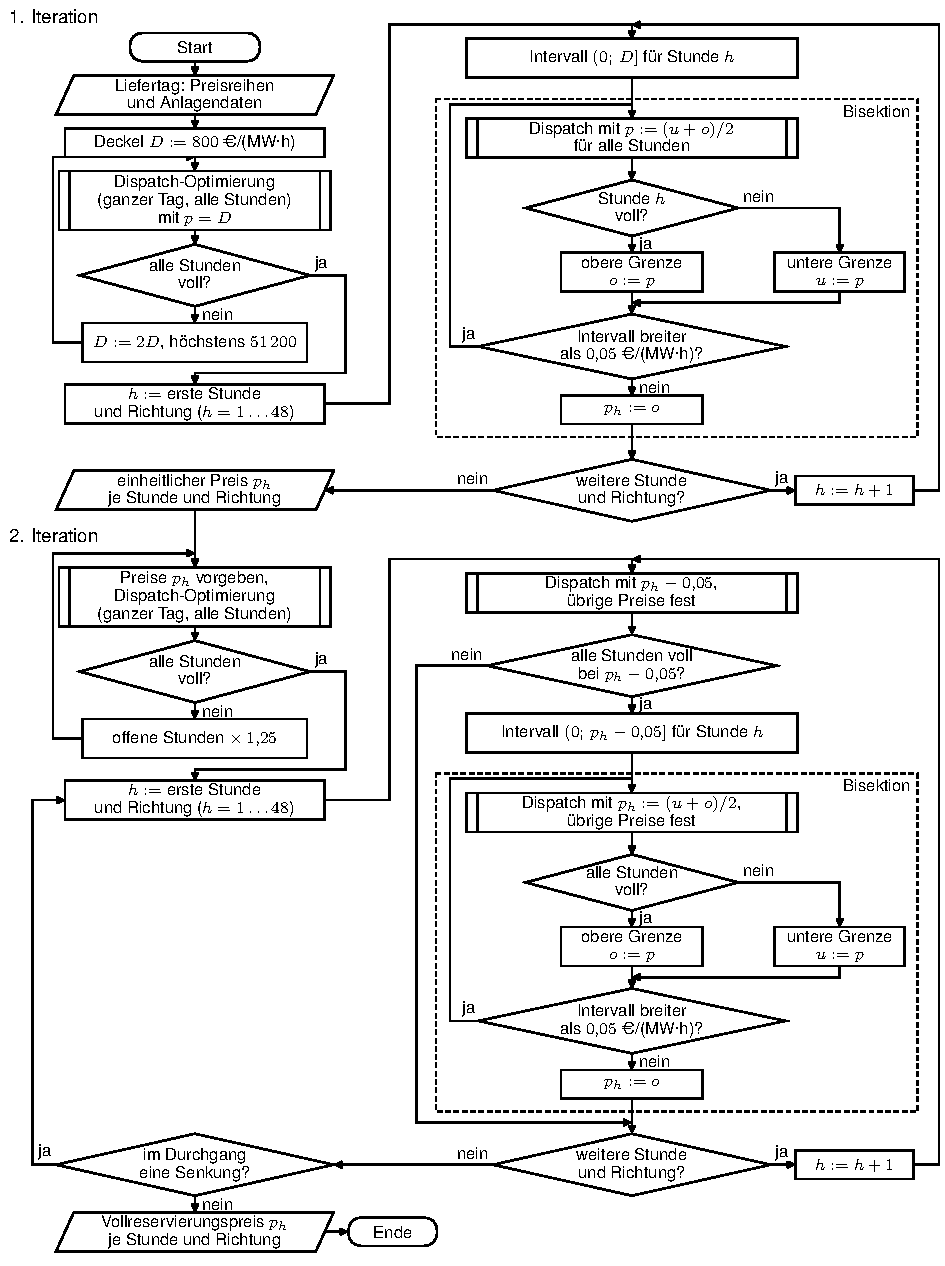
\includegraphics[width=\textwidth]{figures/chapter_3/reservierungspreis_ablauf_gross.pdf}
    \caption{Ablauf der Bestimmung des kurativen Reservierungspreises in zwei Iterationen, Symbole nach DIN 66001. Links bestimmt jede Iteration die Grenzen des Intervalls, rechts halbiert jede Iteration dieses Intervall.}
    \label{fig:reservierungspreis_ablauf_gross}
\end{figure}
